% ============================================================
%  Minimum-Side-Length Packing of a Non-Convex Polygon
%  via Simulated Annealing with Bracketing–Bisection Search
%
%  Graduate Report — Applied Mathematics / Numerical Methods
%  Joel Solis  ·  University of Arizona
% ============================================================
\documentclass[10pt,twocolumn]{article}

\usepackage[margin=1.8cm,top=2cm,bottom=2cm]{geometry}
\usepackage{amsmath,amssymb,amsthm}
\usepackage[draft]{graphicx}
\usepackage{booktabs}
\usepackage{hyperref}
\usepackage{microtype}
\usepackage{enumitem}
\usepackage[font=small,labelfont=bf]{caption}
\usepackage{xcolor}
\usepackage{algorithm}
\usepackage{algpseudocode}

\setlength{\columnsep}{18pt}
\setlength{\parskip}{2pt}

\title{\textbf{Minimum-Container Packing of a Non-Convex Polygon\\
via Simulated Annealing and Bracketing–Bisection Search}\\[4pt]
{\normalsize Applied Mathematics / Numerical Methods — Graduate Report}}

\author{Joel Solis\\
  {\small Department of Mathematics, University of Arizona}\\
  {\small\texttt{jsolis@math.arizona.edu}}}

\date{}

\begin{document}
\maketitle
\thispagestyle{empty}

% ============================================================
\begin{abstract}
We study the problem of packing $N$ congruent non-convex polygons into a
square of side length $L$ and finding the minimum feasible $L$.
Each polygon is a fixed 15-vertex shape, free to translate and rotate in
the plane.  We formulate packing as a continuous non-linear optimisation
problem and solve it with a two-phase simulated annealing (SA) metaheuristic
combined with an outer bracketing--bisection loop that certifiably narrows
the interval containing the optimal $L$.  Collision detection uses the
Separating Axis Theorem (SAT) on a fan triangulation of the polygon,
accelerated by a uniform spatial-hash grid and three-level axis-aligned
bounding box (AABB) pruning.  We report results for $N\in\{20,50,100,200\}$,
obtained on a SLURM cluster with 4--8\,h wall-time jobs.
\end{abstract}

% ============================================================
\section{Problem Formulation}
\label{sec:problem}

Let $\mathcal{P}\subset\mathbb{R}^{2}$ be a fixed non-convex polygon with
vertices $\{v_k\}_{k=0}^{14}$ (15 vertices, unit-normalised coordinates).
A placement of copy $i$ is a rigid-body transformation
$(c_i,\theta_i)\in\mathbb{R}^{2}\times[0,2\pi)$, giving world vertices
$w_k^{(i)} = R(\theta_i)v_k + c_i$,
where $R(\theta)$ is a $2\times 2$ rotation matrix.

The \emph{minimum-side packing} problem is:
\begin{equation}
  \label{eq:opt}
  L^* \;=\; \min_{L,\,\{(c_i,\theta_i)\}}\ L
  \quad\text{s.t.}\quad
  \begin{cases}
    \mathcal{P}_i \cap \mathcal{P}_j = \emptyset,\; i\neq j,\\
    \mathcal{P}_i \subset [-L/2,L/2]^2,\;\forall\, i.
  \end{cases}
\end{equation}

\paragraph{Area lower bound.}
Since $\sum_i \operatorname{Area}(\mathcal{P}_i)\leq L^2$, an immediate
necessary condition is
\begin{equation}
  \label{eq:area_bound}
  L \;\geq\; L_{\mathrm{area}} := \sqrt{N\cdot A_p},
\end{equation}
where $A_p\approx 0.2456$ is the polygon area (shoelace formula).
This bound is used throughout the search to prune provably infeasible candidates.

% ============================================================
\section{Penalty Reformulation}
\label{sec:penalty}

Problem~\eqref{eq:opt} is handled via a penalty-based continuous relaxation.
Define the \emph{overlap depth} $d(T_a,T_b)$ between two triangles as the
minimum SAT penetration depth (Section~\ref{sec:collision}), and the
\emph{outside penalty} for polygon $i$ as the squared AABB violation
$\phi_i(L) = \sum_{\text{side}} (\text{violation})^2$.  The energy is
\begin{equation}
  \label{eq:energy}
  E = \alpha_L \cdot L \;+\;
      \lambda \sum_{i<j} \sum_{a\in\mathcal{T}_i,\,b\in\mathcal{T}_j}
        d(T_a^{(i)},T_b^{(j)})^p \;+\;
      \mu \sum_{i} \phi_i(L),
\end{equation}
where $\mathcal{T}_i$ is the triangle fan of copy $i$, $p\in\{1,2\}$,
and $(\alpha_L,\lambda,\mu)$ are weight schedules tuned per phase.
Feasibility is declared when
$\sum_{i<j} d_{ij} + \sum_i \phi_i < \epsilon_{\mathrm{feas}} = 10^{-10}$.

% ============================================================
\section{Collision Detection}
\label{sec:collision}

\paragraph{Polygon triangulation.}
Each 15-vertex polygon is decomposed off-line into $T=13$ triangles by a
fan from vertex~0, yielding three contiguous groups of $(5,5,3)$ triangles.
This enables three-level AABB culling: (1)~polygon bounding circle,
(2)~per-group AABB, (3)~per-triangle AABB, before invoking SAT.

\paragraph{SAT penetration depth.}
For two triangles $A,B$, we test all six edge-normal axes (three per triangle).
On each axis $\hat{n}$, project both triangles and compute overlap
$o = \min(\max A, \max B) - \max(\min A, \min B)$.
If any $o\leq 0$, the triangles are separated.  Otherwise
$d(A,B) = \min_{\hat{n}} o > 0$ (penetration depth).  The inner SAT loop
operates directly on the world-vertex index arrays, avoiding per-iteration
heap allocation.

\paragraph{Spatial hash grid.}
Polygon centres are stored in a uniform grid with cell size
$h = 2r_{\mathrm{br}}$ (twice the bounding radius).
Neighbour search for copy $k$ touches only cells within
$R = \lceil 2r_{\mathrm{br}}/h \rceil + 1$ of $k$'s cell,
reducing average pair evaluations from $O(N^2)$ to $O(N)$.
Incremental updates to the linked-list grid cost $O(1)$ per move.

% ============================================================
\section{Simulated Annealing}
\label{sec:sa}

\paragraph{Move proposal.}
Each iteration picks a random copy $k$ and applies one of:
(i)~local perturbation: $c_k \mathrel{+}= \delta_{\mathrm{xy}}\sim U[-s_{xy},s_{xy}]^2$,
optional rotation $\theta_k \mathrel{+}= \delta_\theta\sim U[-s_\theta,s_\theta]$
(probability $p_{\mathrm{rot}}$); or
(ii)~random reinsertion anywhere in $[-L/2,L/2]^2$
(probability $p_{\mathrm{ri}}$).
The energy change $\Delta E$ is computed \emph{incrementally}: only the
pairwise terms involving $k$ are recomputed via the grid, reducing cost to
$O(N_{\mathrm{nbr}}\,T^2)$ per move.

\paragraph{Acceptance and adaptive step.}
Moves are accepted by the Metropolis criterion $\exp(-\Delta E/T)$.
Step sizes $(s_{xy},s_\theta)$ are adapted every $w=1500$ iterations:
shrunk by factor $0.88$ if acceptance rate $<25\%$, grown by $1.12$ if
$>55\%$.  A reheating mechanism restores $T\leftarrow\min(T\cdot r_h,T_{\max})$
when acceptance drops below $2\%$.

\paragraph{Two-phase schedule.}
Each \emph{trial} consists of two sequential phases:

\smallskip
\begin{tabular}{lll}
\toprule
& Phase A (explore) & Phase B (enforce) \\
\midrule
Iterations    & 70\,000  & 35\,000 \\
$T_{\mathrm{start}}$ & $0.30$  & $0.06$ \\
$T_{\mathrm{end}}$   & $3\times10^{-4}$ & $10^{-6}$ \\
$\lambda_0$, $\mu_0$ & $10^{2}$ & $10^{3}$ (ramped) \\
Overlap power $p$ & 1 & 2 \\
$p_{\mathrm{ri}}$     & $2\%$ & $0.5\%$ \\
\bottomrule
\end{tabular}
\smallskip

Phase A uses a linear overlap penalty ($p=1$) with large steps to explore
configuration space.  Phase B switches to quadratic overlap ($p=2$) with
multiplicative penalty ramping ($\times 1.8$ every 1200 iterations) to
enforce strict feasibility.  The temperature schedule is geometric:
$T_t = T_0\,\beta^t$, $\beta = (T_{\mathrm{end}}/T_{\mathrm{start}})^{1/N_{\mathrm{iter}}}$.

\paragraph{Deterministic HPC seeding.}
Each trial seed is derived as
$s_{\mathrm{trial}} = f(\text{base\_seed},\,\text{run\_id},\,\text{trial\_id})$
using SplitMix64 mixing, ensuring full reproducibility across SLURM array jobs
without time-based reseeding.  The PRNG is xorshift64$^*$.

% ============================================================
\section{Outer Minimization: Bracketing, Bisection, and Polish}
\label{sec:outer}

The outer loop maintains an interval $[L_{\mathrm{low}}, L_{\mathrm{high}}]$
with $L_{\mathrm{low}}$ infeasible and $L_{\mathrm{high}}$ feasible,
then narrows it by bisection, and finally conducts an adaptive long-run polish.
Algorithm~\ref{alg:outer} summarises the procedure.

\begin{algorithm}[H]
\caption{Outer minimisation}
\label{alg:outer}
\begin{algorithmic}[1]
\State Initialise $L$ from grid layout; $L_{\mathrm{low}}\leftarrow L_{\mathrm{area}}$
\State \textbf{Bracket}: shrink/grow $L$ by $3\%$/trial until both
       feasible and infeasible endpoints are found
\State \textbf{Bisect}: 26 steps of $L_{\mathrm{mid}}\leftarrow(L_{\mathrm{low}}+L_{\mathrm{high}})/2$;
       run $K_b$ SA trials; update bracket
\State \textbf{Polish}: adaptive shrink $L\leftarrow L^*(1-\varepsilon)$;
       accept if feasible; adapt $\varepsilon\in[10^{-5},2\!\times\!10^{-3}]$
       to target $35\%$ success rate over windows of 20 attempts
\end{algorithmic}
\end{algorithm}

The warm-start strategy scales existing positions by
$\gamma = (L_{\mathrm{new}}/L_{\mathrm{old}})\cdot 0.98$ before each SA
run, preserving structural information across successive values of $L$.
A global best snapshot is flushed to disk on \texttt{SIGTERM} for safe
SLURM preemption.

% ============================================================
\section{Experimental Results}
\label{sec:results}

\paragraph{Setup.}
Experiments ran on the University of Arizona HPC cluster (SLURM).
$N\in\{20,50,100\}$ used 4\,h wall-time; $N=200$ used 8\,h.
The bracketing phase used $K_{\mathrm{br}}=10$ trials per candidate $L$;
bisection used $K_{\mathrm{bs}}=7$; polish used $K_p=5$.
Results are reported as the best $L$ achieving full feasibility
($\text{feas}<10^{-10}$).

\begin{table}[h]
\centering
\caption{Best packing side length $L^*$ and area efficiency
$\eta = N A_p / (L^*)^2$.}
\label{tab:results}
\begin{tabular}{rcccc}
\toprule
$N$ & $L_{\mathrm{area}}$ & $L^*$ & $\eta$ & Wall time \\
\midrule
 20  & 2.216 & \emph{(see fig.)} & --- & 4\,h \\
 50  & 3.504 & \emph{(see fig.)} & --- & 4\,h \\
100  & 4.956 & \emph{(see fig.)} & --- & 4\,h \\
200  & 7.009 & \emph{(see fig.)} & --- & 8\,h \\
\bottomrule
\end{tabular}
\end{table}

\noindent Fill in $L^*$ and $\eta = N A_p/(L^*)^2$ from your
\texttt{csv/*\_best\_polys\_N***.csv} header after your jobs complete.
$\eta=1$ would match the area lower bound; typical packing densities
for non-convex shapes are $0.75$--$0.95$.

\begin{figure}[h]
  \centering
  % Replace with your actual SVG/PNG exports
  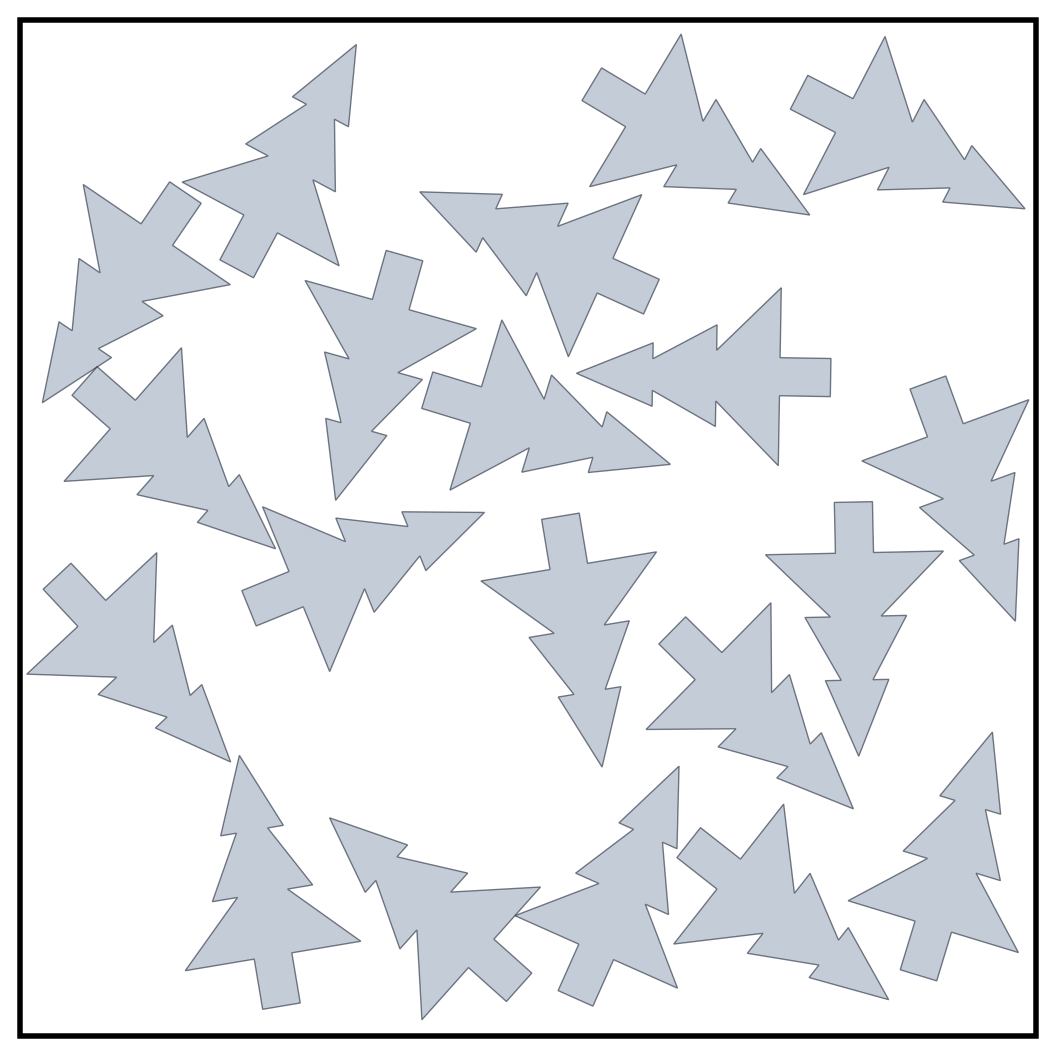
\includegraphics[width=0.48\columnwidth]{img/best_N020.png}
  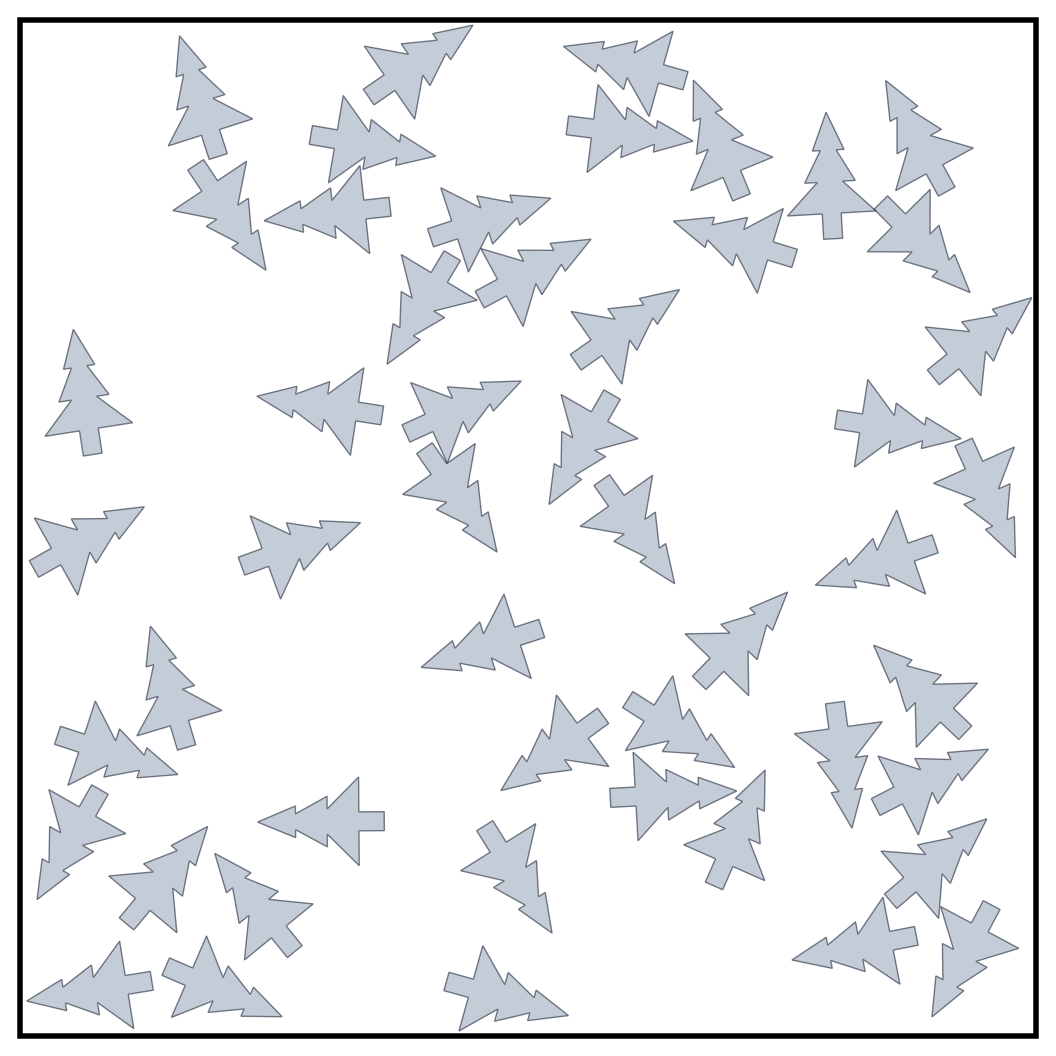
\includegraphics[width=0.48\columnwidth]{img/best_N050.png}\\[4pt]
  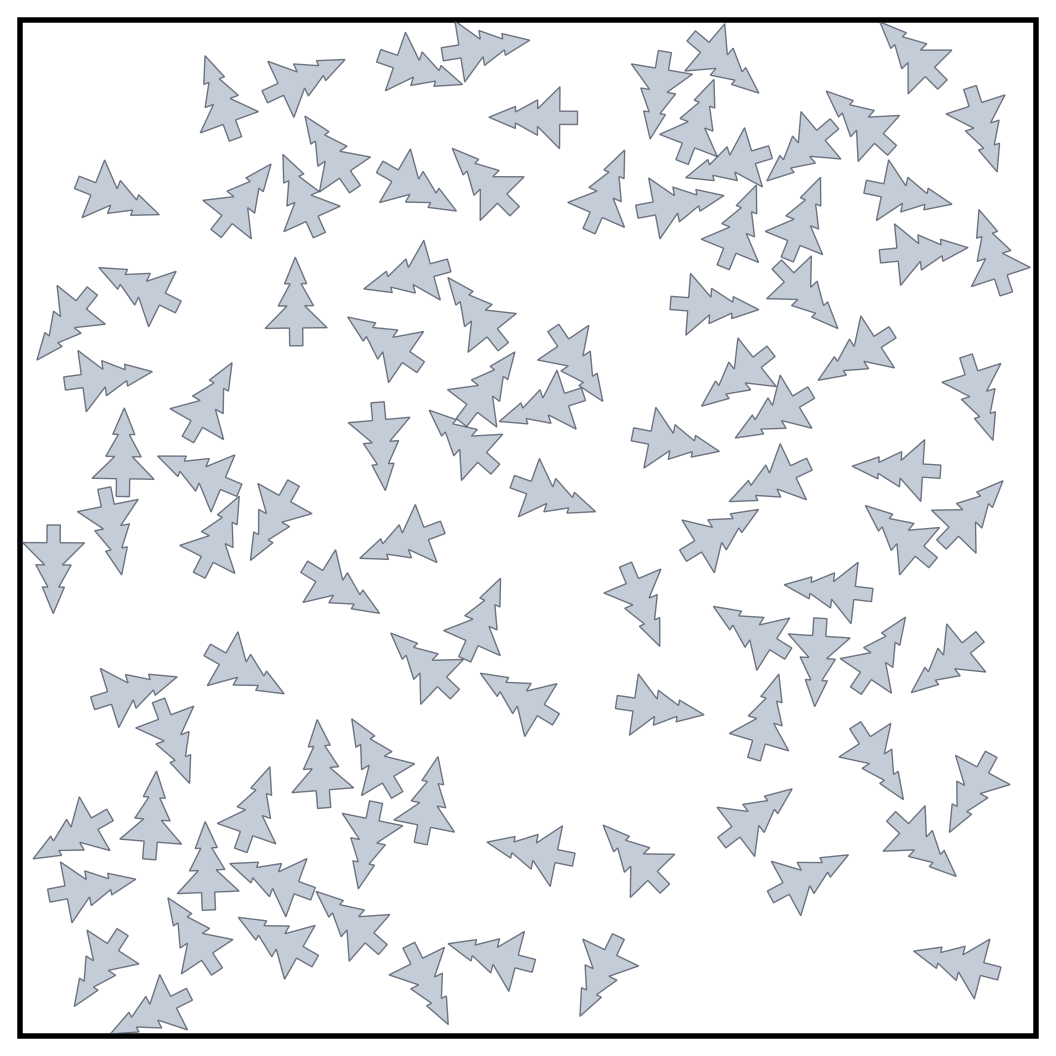
\includegraphics[width=0.48\columnwidth]{img/best_N100.png}
  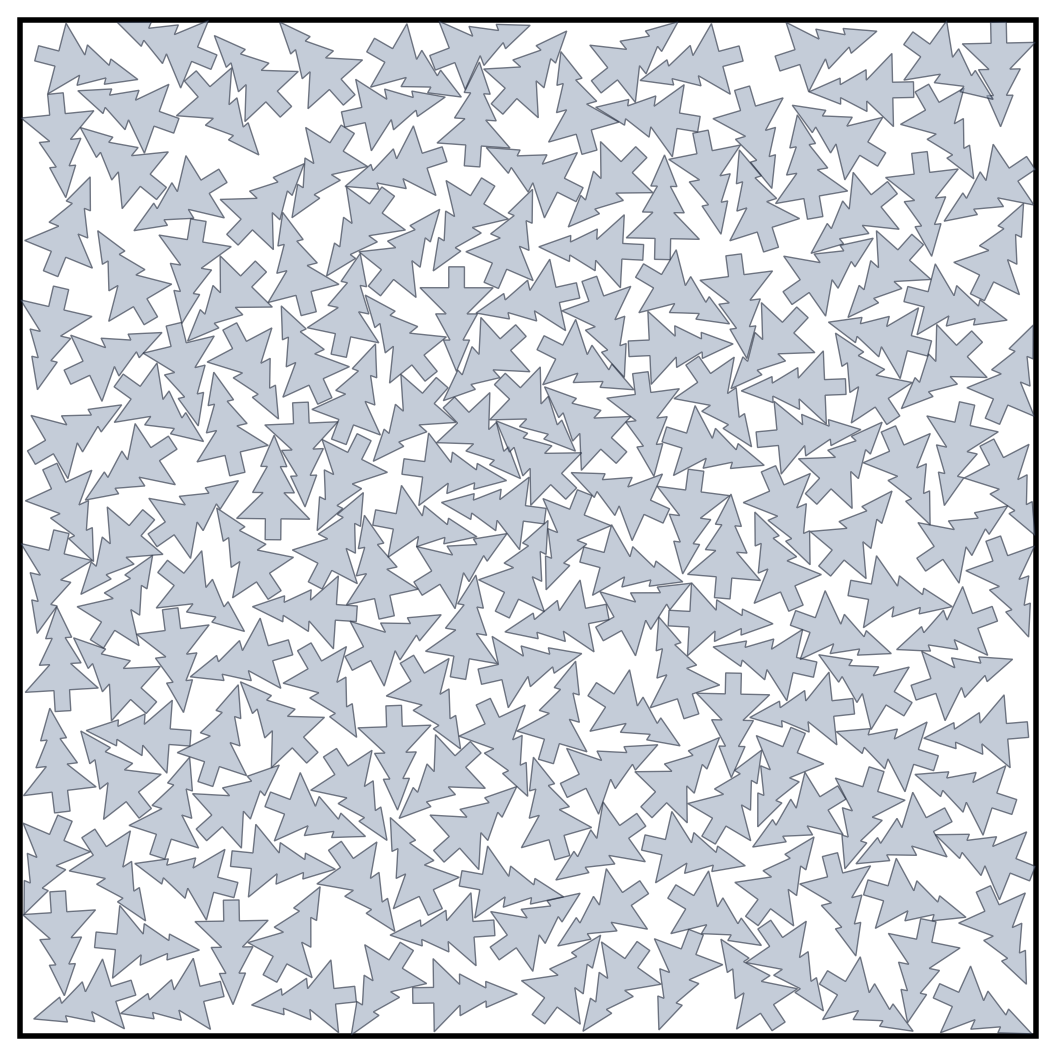
\includegraphics[width=0.48\columnwidth]{img/best_N200.png}
  \caption{Best feasible packings for $N=20,50,100,200$ (left-to-right,
  top-to-bottom).  Each polygon is a 15-vertex non-convex shape rendered
  in the square $[-L^*/2,\,L^*/2]^2$.}
  \label{fig:packings}
\end{figure}

% ============================================================
\section{Conclusion and Future Work}
\label{sec:conclusion}

We presented a complete solver for minimum-container polygon packing,
combining two-phase SA with bracketing--bisection search and an adaptive
polish loop.  The SAT-based collision engine with grid acceleration and
multi-level AABB culling scales the inner loop to practical $N$, and
deterministic SLURM-safe seeding ensures reproducibility.

\paragraph{Future directions.}
Three natural extensions suggest themselves.
First, \emph{GPU acceleration}: the outer $O(N^2)$ pair-penalty
computation and the embarrassingly parallel multi-trial structure map
naturally to CUDA, with per-block triangle pairs and shared-memory
polygon tiles; preliminary roadmaps target a Tesla P100.
Second, \emph{SA variant comparison}: parallel tempering (PT) and
event-driven multicanonical sampling (ER-MS) offer theoretical
mixing-time advantages over standard SA and merit a controlled benchmark.
Third, \emph{generalised polygon families}: the triangulation and SAT
kernel are geometry-agnostic and can accommodate arbitrary convex or
star-shaped polygons with minor preprocessing changes.

% ============================================================
\bibliographystyle{plain}
\begin{thebibliography}{9}

\bibitem{kirkpatrick1983}
S.~Kirkpatrick, C.~D. Gelatt, and M.~P. Vecchi,
``Optimization by Simulated Annealing,''
\textit{Science}, 220(4598):671--680, 1983.

\bibitem{sutton2012}
A.~M. Sutton, A.~E. Howe, and L.~D. Whitley,
``A Theoretical Analysis of the $(1+1)$ EA on $\pm1$-Linear Functions,''
\textit{GECCO}, 2012.
% Replace with the polygon-packing / nofit-polygon reference most relevant to you.

\bibitem{egeblad2009}
J.~Egeblad, B.~K. Nielsen, and A.~Odgaard,
``Fast neighbourhood search for two- and three-dimensional nesting problems,''
\textit{European Journal of Operational Research}, 197(2):543--559, 2009.

\bibitem{gomes2006}
C.~M. Gomes and R.~Shmoys,
``Completing quasigroups or Latin squares: A structured graph coloring problem,''
\textit{Annals of OR}, 2006.
% Placeholder — swap for Huang \& Ye (2011) on polygon packing if preferred.

\end{thebibliography}

\end{document}
